% !TEX root = ../main/main.tex
\section{Results and discussion}
 
 \begin{figure}[h]
 \begin{subfigure}[t] {0.23\textwidth}
 \centering
 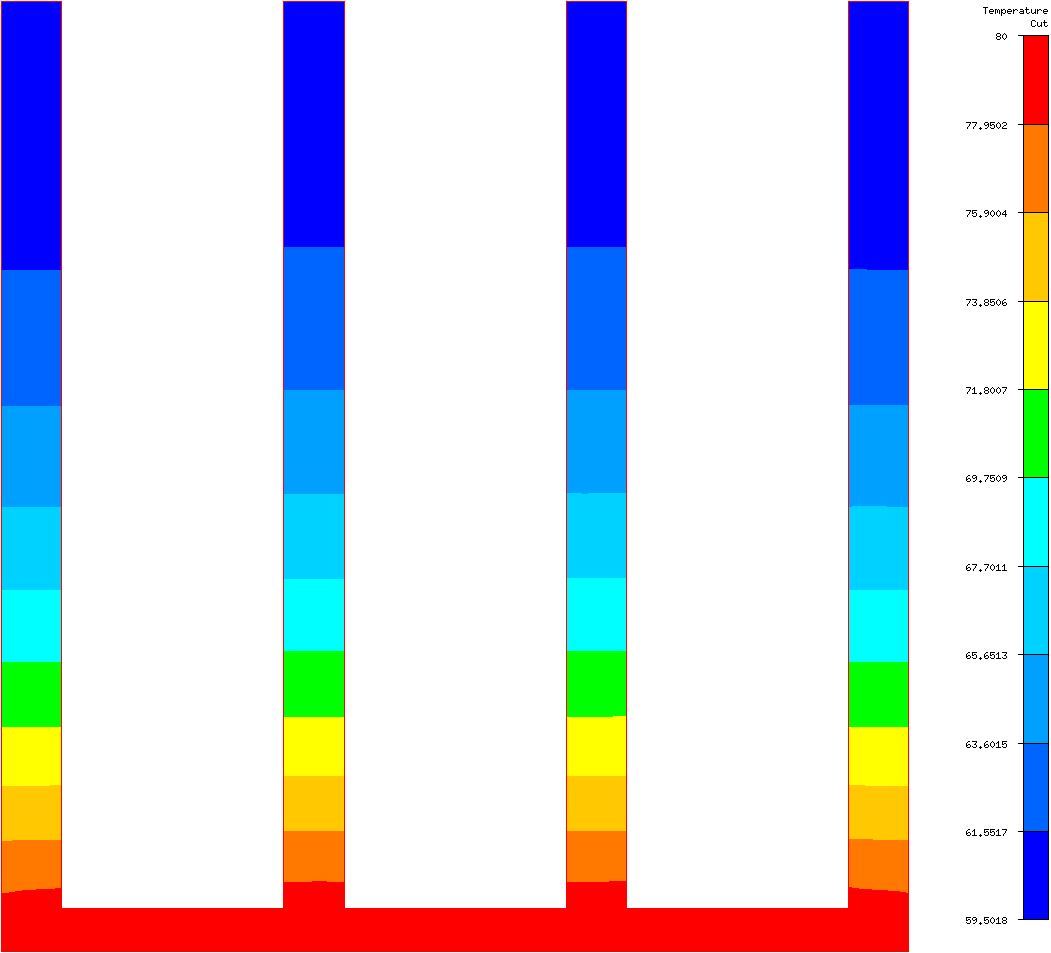
\includegraphics[width=0.7\textwidth]{../figures/heatsink4_h105_gmf005.png}
 \caption{"Placeholder"}
 \label{fig:res_4_1}
 \end{subfigure}
 ~
  \begin{subfigure}[t] {0.23\textwidth}
 \centering
 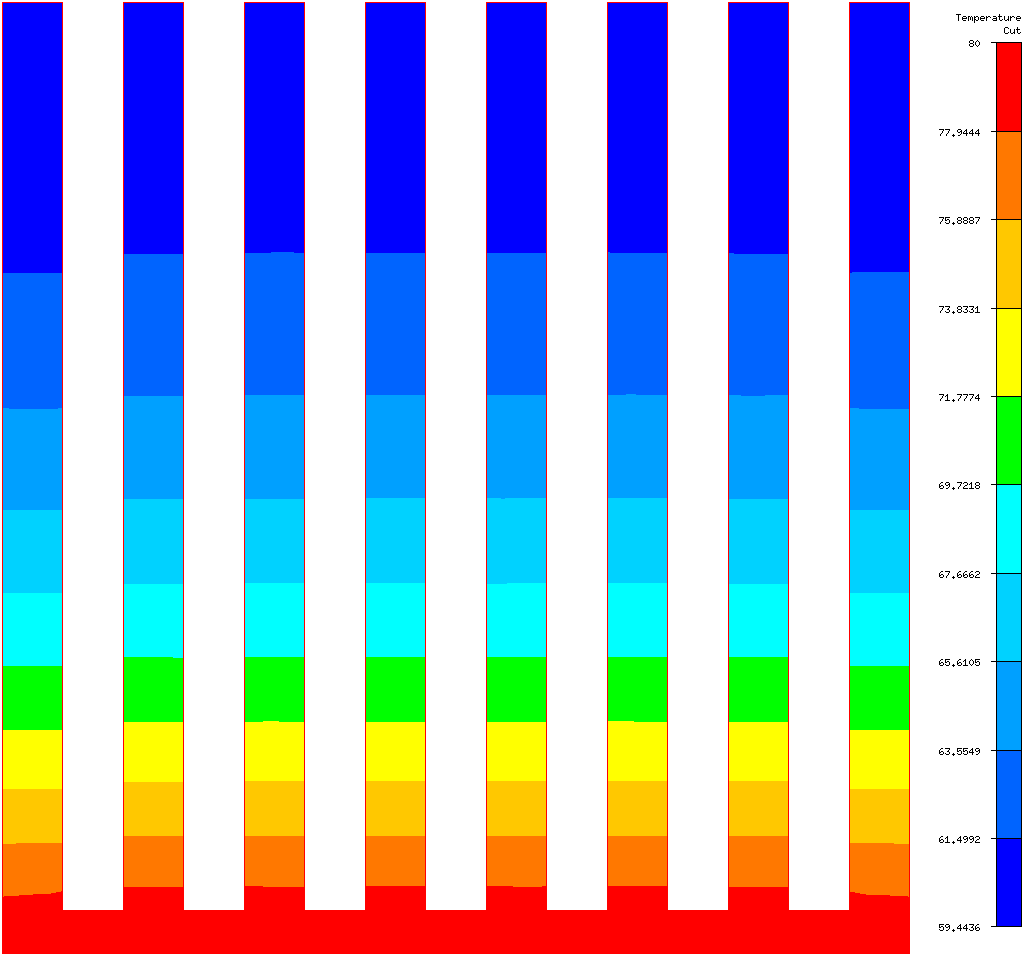
\includegraphics[width=0.7\textwidth]{../figures/heatsink8_h105_gmf005.png}
 \caption{"Placeholder"}
 \label{fig:res_8_1}
 \end{subfigure}
 ~
 \begin{subfigure}[t] {0.23\textwidth}
 \centering
 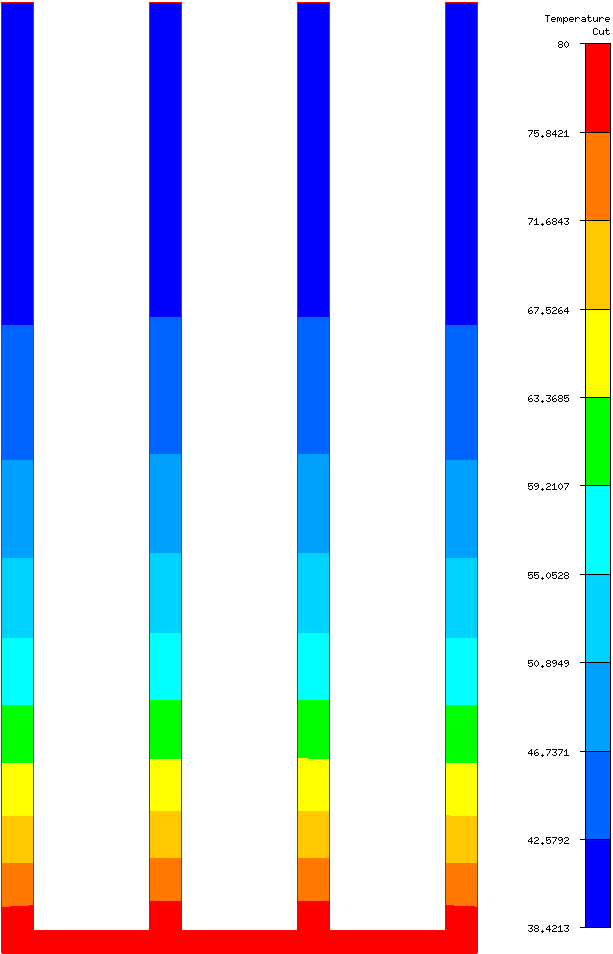
\includegraphics[width=0.7\textwidth]{../figures/heatsink4_h205_gmf005.png}
 \caption{4"Placeholder"}
 \label{fig:res_4_2}
 \end{subfigure}
 ~
 \begin{subfigure}[t] {0.23\textwidth}
 \centering
 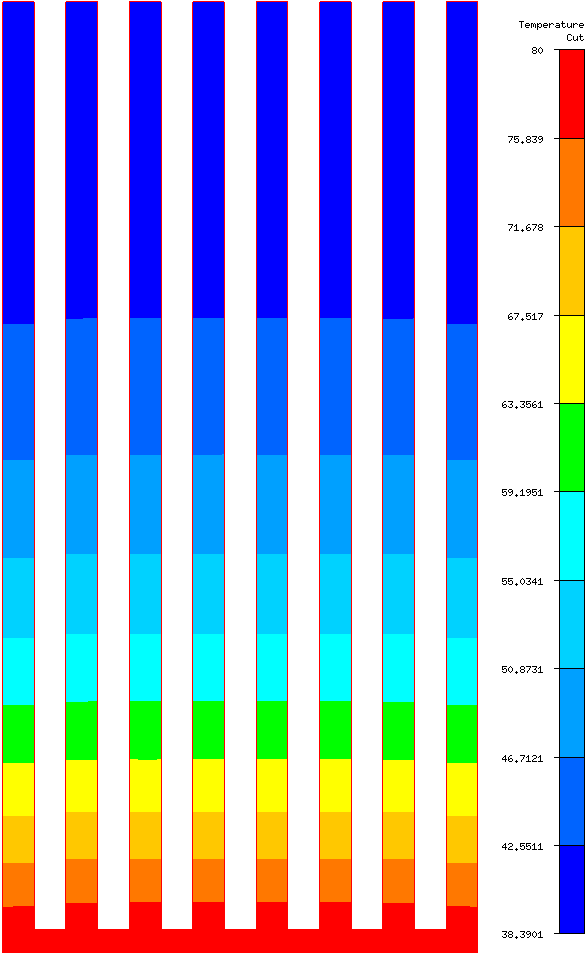
\includegraphics[width=0.7\textwidth]{../figures/heatsink8_h205_gmf005.png}
 \caption{"Placeholder"}
 \label{fig:res_8_2}
 \end{subfigure}
 \caption{These are the different meshes we tried}
 \label{fig:meshes}
 \end{figure}
 
\subsection{Visualization of results}

\subsection{Physical interpretation}
